\documentclass[a4paper,12pt]{Latex/Classes/PhDthesisPSnPDF}
\usepackage[utf8]{inputenc}
\usepackage{amsthm}
\usepackage{graphicx}
\usepackage{subcaption, siunitx, booktabs}
\usepackage{caption}

% \usepackage[spanish]{babel}
% \input{body/preamble/preamble.Rnw}
% This file contains macros that can be called up from connected TeX files
% It helps to summarise repeated code, e.g. figure insertion (see below).

%%%%%%%%%%%%%%%%%%%%%%%%%%%%%%%%%%%%%%%%%%%%%%
%            Colores de la UNAM              %
%%%%%%%%%%%%%%%%%%%%%%%%%%%%%%%%%%%%%%%%%%%%%%
%Azul Pantone 541  -->(0,63,119) RGB
\definecolor{Azul}{RGB}{128,0,0}

%Oro Pantone 460  -->(234,221,150) RGB
\definecolor{Oro}{RGB}{234,221,150}


%%%%%%%%%%%%%%%%%%%%%%%%%%%%%%%%%%%%%%%%%%%%%%
%            Comandos para líneas            %
%%%%%%%%%%%%%%%%%%%%%%%%%%%%%%%%%%%%%%%%%%%%%%
%Se define un comando \colorvrule para hacer líneas verticales de color con 3 argumentos: color, ancho, alto
\newcommand{\colorvrule}[3]{
\begingroup\color{#1}\vrule width#2 height#3
\endgroup}

%Se define un comando \colorhrule para hacer líneas horizontales de color con 2 argumentos: color, ancho
\newcommand{\colorhrule}[2]{
\begingroup\color{#1}\hrule height#2
\endgroup}

%%%%%%%%%%%%%%%%%%%%%%%%%%%%%%%%%%%%%%%%%%%%%%
%          Comando para derivadas            %
%%%%%%%%%%%%%%%%%%%%%%%%%%%%%%%%%%%%%%%%%%%%%%
\newcommand{\derivada}[3][]{\ensuremath{\dfrac{\mbox{d}^{#1}#2}{\mbox{d}#3^{#1}}}} 
%primer argumento(opcional): orden de la derivada
%segundo argumento: función a derivar
%tercer argumento: variable respecto a la que se deriva


%%%%%%%%%%%%%%%%%%%%%%%%%%%%%%%%%%%%%%%%%%%%%%
%       Comando para la exponencial          %
%%%%%%%%%%%%%%%%%%%%%%%%%%%%%%%%%%%%%%%%%%%%%%
\newcommand{\e}[1][]{\ensuremath{\mbox{e}^{#1}}}
%primer argumento(opcional): exponente de la exponencial




% insert a centered figure with caption and description
% parameters 1:filename, 2:title, 3:description and label
\newcommand{\figuremacro}[3]{
	\begin{figure}[htbp]
		\centering
		\includegraphics[width=1\textwidth]{#1}
		\caption[#2]{\textbf{#2} - #3}
		\label{condicion}
	\end{figure}
}

% insert a centered figure with caption and description AND WIDTH
% parameters 1:filename, 2:title, 3:description and label, 4: textwidth
% textwidth 1 means as text, 0.5 means half the width of the text
\newcommand{\figuremacroW}[4]{
	\begin{figure}[htbp]
		\centering
		\includegraphics[width=#4\textwidth]{#1}
		\caption[#2]{\textbf{#2} - #3}
		\label{#1}
	\end{figure}
}

% inserts a figure with wrapped around text; only suitable for NARROW figs
% o is for outside on a double paged document; others: l, r, i(inside)
% text and figure will each be half of the document width
% note: long captions often crash with adjacent content; take care
% in general: above 2 macro produce more reliable layout
\newcommand{\figuremacroN}[3]{
	\begin{wrapfigure}{o}{0.5\textwidth}
		\centering
		\includegraphics[width=0.48\textwidth]{#1}
		\caption[#2]{{\small\textbf{#2} - #3}}
		\label{#1}
	\end{wrapfigure}
}

% predefined commands by Harish
\newcommand{\PdfPsText}[2]{
  \ifpdf
     #1
  \else
     #2
  \fi
}

\newcommand{\IncludeGraphicsH}[3]{
  \PdfPsText{\includegraphics[height=#2]{#1}}{\includegraphics[bb = #3, height=#2]{#1}}
}

\newcommand{\IncludeGraphicsW}[3]{
  \PdfPsText{\includegraphics[width=#2]{#1}}{\includegraphics[bb = #3, width=#2]{#1}}
}

\newcommand{\InsertFig}[3]{
  \begin{figure}[!htbp]
    \begin{center}
      \leavevmode
      #1
      \caption{#2}
      \label{#3}
    \end{center}
  \end{figure}
}







%%% Local Variables:
%%% mode: latex
%%% TeX-master: "~/Documents/LaTeX/CUEDThesisPSnPDF/thesis"
%%% End:
 
\newtheorem{teorema}{Teorema}
\newtheorem{definicion}{Definición}
% \showboxdepth=5
% \showboxbreadth=5
%%%%%%%%%%%%%%%%%%%%%%%%%%%%%%%%%%%%%%%%%%%%%%%%%%%%%%%%%%%%%%%%%%%%%%%%%%%%%%%%
%                                   DATOS                                      %
%%%%%%%%%%%%%%%%%%%%%%%%%%%%%%%%%%%%%%%%%%%%%%%%%%%%%%%%%%%%%%%%%%%%%%%%%%%%%%%%
\title{Evaluación de la Eficacia de una estrategia de trading basada en Modelo Lineal Generalizado}
\author{Rodrigo Alejandro Serrano Morales} 
\facultad{Facultad de Ciencias Económicas y Sociales\\
Escuela de Estadística y Ciencias Actuariales}                % Nombre de la facultad/escuela
\escudofacultad{images/faces} % Aquí ponen la ruta y nombre del escudo de su facultad, actualmente, la carpeta Latex/Classes/Escudos cuenta con los siguientes escudos:
% "fi_azul" Facultad de ingenieria en color azul
% "fi_negro" Facultad de ingenieria en color negro
% "fc_azul" Facultad de ciencias en color azul
% "fc_negro" Facultad de ciencias en color negro
% Se agradecen sus aportaciones de escudos a jebus.velazquez@gmail.com

\degree{Licenciado en Ciencias Actuariales}        % Carrera
\director{Prof. Jonattan Ramos \& Prof. Eloy Eligon}               % Director de tesis
\degreedate{Marzo 2019}                           % Año de la fecha del examen
\lugar{Caracas}                        % Lugar

%\portadafalse                              % Portada en NEGRO, descomentar y comentar la línea siguiente si se quiere utilizar
\portadatrue                                % Portada en COLOR



%% Opciones del posgrado (descomentar si las necesitan)
	%\posgradotrue                                                    
	%\programa{programa de maestría y doctorado en ingeniería}
	%\campo{Ingeniería Eléctrica - Control}
	%% En caso de que haya comité tutor
	%\comitetrue
	%\ctutoruno{Dr. Emmet L. Brown}
	%\ctutordos{Dr. El Doctor}
%% Datos del jurado                             
	%\presidente{Dr. 1}
	%\secretario{Dr. 2}
	%\vocal{Dr. 3}
	%\supuno{Dr. 4}
	%\supdos{Dr. 5}
	%\institucion{el Instituto de Ingeniería, UNAM}

\keywords{tesis,autor,tutor,etc}            % Palablas clave para los metadatos del PDF
\subject{tema_1,tema_2}                     % Tema para metadatos del PDF  

%%%%%%%%%%%%%%%%%%%%%%%%%%%%%%%%%%%%%%%%%%%%%%%%%%%%%
%                   PORTADA                         %
%%%%%%%%%%%%%%%%%%%%%%%%%%%%%%%%%%%%%%%%%%%%%%%%%%%%%
\usepackage{Sweave}
\begin{document}
\Sconcordance{concordance:main.tex:main.Rnw:%
1 64 1 1 0 14 1}
\Sconcordance{concordance:main.tex:./body/introduccion/introduccion.Rnw:ofs 80:%
1 11 1}
\Sconcordance{concordance:main.tex:./body/chapter1/chapter1.Rnw:ofs 92:%
1 43 1}
\Sconcordance{concordance:main.tex:./body/chapter2/chapter2.Rnw:ofs 136:%
1 255 1 1 18 1 2 17 1}
\Sconcordance{concordance:main.tex:./body/chapter3/chapter3.Rnw:ofs 411:%
1 95 1 1 64 3 1 2 2 32 1}
\Sconcordance{concordance:main.tex:./body/chapter4/chapter4.Rnw:ofs 545:%
1 15 1 1 14 3 1 2 2 13 1 1 8 1 3 7 1 1 8 1 2 4 1 1 74 2 1 1 3 1 2 8 1 1 %
3 1 2 8 1 1 3 1 2 8 1 1 12 5 1 1 9 1 2 12 1 1 14 1 2 9 1 1 3 1 2 13 1 1 %
7 1 2 4 1 1 7 3 1 1 7 1 2 22 1 1 3 9 0 1 2 1 1 1 32 1 2 8 0 1 1 7 0 1 2 %
9 0 1 1 10 0 1 2 12 1 1 7 12 0 1 2 3 1 1 6 12 0 1 2 3 1 1 6 12 0 1 2 4 %
1 1 6 12 0 1 2 3 1 1 6 12 0 1 2 4 1 1 6 12 0 1 2 7 1 1 37 2 1 1 2 15 0 %
1 2 3 1 1 26 5 1 1 9 1 2 4 1 1 24 3 1 1 9 1 2 15 1 1 17 2 1 1 2 14 0 1 %
2 3 1 1 27 2 1 1 2 11 0 1 2 2 1}
\Sconcordance{concordance:main.tex:./body/conclusion/conclusion.Rnw:ofs 976:%
1 7 1 1 20 3 1 1 6 1 2 15 1}
\Sconcordance{concordance:main.tex:./body/anexos/anexos.Rnw:ofs 1005:%
1 9 1 1 2 12 0 1 2 3 1 1 2 12 0 1 2 2 1 1 2 12 0 1 2 5 1 1 2 12 0 1 2 3 %
1 1 2 12 0 1 2 2 1 1 2 12 0 1 2 6 1 1 2 12 0 1 2 3 1 1 2 12 0 1 2 3 1 1 %
2 12 0 1 2 5 1 1 2 12 0 1 2 3 1 1 2 12 0 1 2 2 1 1 2 12 0 1 2 6 1 1 2 %
12 0 1 2 3 1 1 2 12 0 1 2 2 1 1 2 12 0 1 2 5 1 1 2 12 0 1 2 3 1 1 2 12 %
0 1 2 2 1 1 2 12 0 1 2 6 1 1 2 12 0 1 2 4 1 1 2 12 0 1 2 2 1 1 2 12 0 1 %
2 5 1 1 2 12 0 1 2 3 1 1 2 12 0 1 2 2 1 1 2 12 0 1 2 1 1}
\Sconcordance{concordance:main.tex:./body/bibliografia/bibliografia.Rnw:ofs 1432:%
1 37 1}
\Sconcordance{concordance:main.tex:main.Rnw:ofs 1470:%
88 1 1}


\maketitle									% Se redefinió este comando en el archivo de la clase para generar automáticamente la portada a partir de los datos

\newpage\renewcommand{\thepage}{\arabic{page}}\setcounter{page}{1} 

% !TeX root = ./main.Rnw
%\SweaveUTF8

\begin{dedication}
Dedicado a mis padres y a mi hermana, por ser los pilares de mi vida y ser mi motivo de haber cumplido esta meta.
\end{dedication}
% !TeX root = ./main.Rnw
%\SweaveUTF8
\newpage
\chapter*{Agradecimientos}

Agradecimientos




  \begin{flushright}
  \textbf{Gracias}
  \end{flushright}

\tableofcontents
\listoffigures
\listoftables


% !TeX root = ./main.Rnw
%\SweaveUTF8

\chapter*{Introducción}
\addcontentsline{toc}{chapter}{Introduccion}

Las economías de países latinoamericanos son reconocidas históricamente por depender en gran magnitud del comercio de sus materias primas, lo cual hace que el comercio con dichos commodities resulte de gran impacto para el gasto fiscal y para la balanza de pagos, esto deja como consecuencia, la necesidad de los actores económicos de estudiar el riesgo a profundidad para poder evitar resultados que reduzcan sus retornos positivos.\\ 

% \SweaveInput{body/chapter1/chapter1.Rnw}
% \SweaveInput{body/chapter2/chapter2.Rnw}
% \SweaveInput{body/chapter3/chapter3.Rnw}
% !TeX root = ./main.Rnw
%\SweaveUTF8

\chapter{Análisis de Resultados}

En el presente capítulo se realiza la descripción de los resultados obtenidos despues de la aplicación del método propuesto para la estrategia. De igual modo, se presentan los resultados arrojados por las pruebas de Backtesting simulando las entradas y salidas.

\section{Resultados del modelo}


En la figura -- se describen los resultados de los parámetros arrojados por la regresión logística en los 6 períodos de entrenamiento para la serie del S\&P500.

\captionof{table}{Resumen del modelo para cada período de entrenamiento utilizando S\&P500}
\captionof*{table}{Período de entrenamiento 2009 - 2012}
% latex table generated in R 3.5.2 by xtable 1.8-3 package
% Fri Feb  8 14:41:47 2019
\begin{table}[ht]
\centering
\begin{tabular}{rrrrr}
  \hline
 & Estimate & Std. Error & z value & Pr($>$$|$z$|$) \\ 
  \hline
(Intercept) & -0.3599 & 0.0645 & -5.58 & 0.0000 \\ 
  PC1 & -0.0146 & 0.0181 & -0.81 & 0.4183 \\ 
  PC2 & -0.0134 & 0.0203 & -0.66 & 0.5085 \\ 
  PC3 & 0.0050 & 0.0327 & 0.15 & 0.8779 \\ 
  PC4 & 0.0873 & 0.0353 & 2.47 & 0.0135 \\ 
  PC5 & -0.0222 & 0.0373 & -0.60 & 0.5514 \\ 
  PC6 & -0.0158 & 0.0425 & -0.37 & 0.7100 \\ 
  PC7 & 0.1057 & 0.0484 & 2.18 & 0.0289 \\ 
   \hline
\end{tabular}
\end{table}\captionof*{table}{Período de entrenamiento 2009 - 2013}
% latex table generated in R 3.5.2 by xtable 1.8-3 package
% Fri Feb  8 14:41:47 2019
\begin{table}[ht]
\centering
\begin{tabular}{rrrrr}
  \hline
 & Estimate & Std. Error & z value & Pr($>$$|$z$|$) \\ 
  \hline
(Intercept) & -0.4093 & 0.0580 & -7.06 & 0.0000 \\ 
  PC1 & 0.0222 & 0.0165 & 1.35 & 0.1785 \\ 
  PC2 & -0.0072 & 0.0182 & -0.40 & 0.6925 \\ 
  PC3 & 0.0169 & 0.0290 & 0.58 & 0.5596 \\ 
  PC4 & 0.0537 & 0.0307 & 1.75 & 0.0800 \\ 
  PC5 & 0.0237 & 0.0336 & 0.71 & 0.4797 \\ 
  PC6 & 0.0393 & 0.0365 & 1.08 & 0.2817 \\ 
  PC7 & -0.1222 & 0.0414 & -2.95 & 0.0032 \\ 
   \hline
\end{tabular}
\end{table}\captionof*{table}{Período de entrenamiento 2009 - 2014}
% latex table generated in R 3.5.2 by xtable 1.8-3 package
% Fri Feb  8 14:41:47 2019
\begin{table}[ht]
\centering
\begin{tabular}{rrrrr}
  \hline
 & Estimate & Std. Error & z value & Pr($>$$|$z$|$) \\ 
  \hline
(Intercept) & -0.2806 & 0.0527 & -5.33 & 0.0000 \\ 
  PC1 & 0.0464 & 0.0156 & 2.98 & 0.0029 \\ 
  PC2 & 0.0260 & 0.0173 & 1.50 & 0.1334 \\ 
  PC3 & 0.0755 & 0.0265 & 2.85 & 0.0043 \\ 
  PC4 & -0.0440 & 0.0271 & -1.63 & 0.1039 \\ 
  PC5 & -0.0449 & 0.0314 & -1.43 & 0.1527 \\ 
  PC6 & -0.0774 & 0.0324 & -2.39 & 0.0168 \\ 
  PC7 & -0.1044 & 0.0384 & -2.72 & 0.0065 \\ 
   \hline
\end{tabular}
\end{table}\captionof*{table}{Período de entrenamiento 2009 - 2015}
% latex table generated in R 3.5.2 by xtable 1.8-3 package
% Fri Feb  8 14:41:47 2019
\begin{table}[ht]
\centering
\begin{tabular}{rrrrr}
  \hline
 & Estimate & Std. Error & z value & Pr($>$$|$z$|$) \\ 
  \hline
(Intercept) & -0.1756 & 0.0490 & -3.58 & 0.0003 \\ 
  PC1 & -0.0670 & 0.0151 & -4.43 & 0.0000 \\ 
  PC2 & 0.0259 & 0.0168 & 1.54 & 0.1239 \\ 
  PC3 & -0.1284 & 0.0238 & -5.39 & 0.0000 \\ 
  PC4 & -0.0246 & 0.0270 & -0.91 & 0.3622 \\ 
  PC5 & -0.0647 & 0.0295 & -2.19 & 0.0287 \\ 
  PC6 & -0.1049 & 0.0309 & -3.40 & 0.0007 \\ 
  PC7 & -0.1040 & 0.0364 & -2.86 & 0.0042 \\ 
   \hline
\end{tabular}
\end{table}\captionof*{table}{Período de entrenamiento 2009 - 2016}
% latex table generated in R 3.5.2 by xtable 1.8-3 package
% Fri Feb  8 14:41:47 2019
\begin{table}[ht]
\centering
\begin{tabular}{rrrrr}
  \hline
 & Estimate & Std. Error & z value & Pr($>$$|$z$|$) \\ 
  \hline
(Intercept) & -0.1306 & 0.0456 & -2.86 & 0.0042 \\ 
  PC1 & -0.0643 & 0.0139 & -4.61 & 0.0000 \\ 
  PC2 & 0.0319 & 0.0157 & 2.03 & 0.0423 \\ 
  PC3 & -0.1211 & 0.0217 & -5.58 & 0.0000 \\ 
  PC4 & -0.0209 & 0.0254 & -0.82 & 0.4101 \\ 
  PC5 & -0.0352 & 0.0274 & -1.28 & 0.1988 \\ 
  PC6 & -0.0993 & 0.0300 & -3.31 & 0.0009 \\ 
  PC7 & -0.0901 & 0.0342 & -2.63 & 0.0084 \\ 
   \hline
\end{tabular}
\end{table}\newpage
\captionof*{table}{Período de entrenamiento 2009 - 2017}
% latex table generated in R 3.5.2 by xtable 1.8-3 package
% Fri Feb  8 14:41:47 2019
\begin{table}[ht]
\centering
\begin{tabular}{rrrrr}
  \hline
 & Estimate & Std. Error & z value & Pr($>$$|$z$|$) \\ 
  \hline
(Intercept) & -0.1148 & 0.0427 & -2.69 & 0.0072 \\ 
  PC1 & 0.0629 & 0.0130 & 4.85 & 0.0000 \\ 
  PC2 & 0.0334 & 0.0144 & 2.31 & 0.0208 \\ 
  PC3 & 0.0977 & 0.0199 & 4.90 & 0.0000 \\ 
  PC4 & 0.0053 & 0.0231 & 0.23 & 0.8202 \\ 
  PC5 & 0.0223 & 0.0255 & 0.87 & 0.3816 \\ 
  PC6 & -0.0584 & 0.0275 & -2.12 & 0.0340 \\ 
  PC7 & -0.0725 & 0.0319 & -2.28 & 0.0228 \\ 
   \hline
\end{tabular}
\end{table}
Se observa que para todos los períodos el ACP arroja componentes que recogen el 85\% de la variación. También se aprecia que a medida que aumentamos los años de entrenamiento el número de p-valores menores que 0.05 aumentan, insinuando que mientras más observaciones para entrenar el modelo, mayor será la asociación entre los componentes y la capacidad de predecir el retorno objetivo.
\\

\begin{center}
\captionof{table}{Resumen de resultados de aplicar el modelo en la data de prueba para los 5 índices}
% latex table generated in R 3.5.2 by xtable 1.8-3 package
% Fri Feb  8 14:41:47 2019
\begin{table}[ht]
\centering
\begin{tabular}{cccccc}
  \hline
 & S\&P\_500 & NASDAQ & NIKKEI\_225 & FTSE\_100 & BOVESPA \\ 
  \hline
True Buys & 21 & 61 & 99 & 53 & 128 \\ 
  False Buys & 32 & 98 & 127 & 62 & 164 \\ 
  N° trades & 53 & 159 & 226 & 115 & 292 \\ 
  Accuracy & 60.38\% & 61.64\% & 56.19\% & 53.91\% & 56.16\% \\ 
  Accumulative Return & 2.57\% & 5.17\% & 2.21\% & 0.70\% & 0.80\% \\ 
  Max Drawdown & 1.13\% & 1.37\% & 3.46\% & 1.42\% & 5.64\% \\ 
   \hline
\end{tabular}
\end{table}\end{center}
 
 
 
 
\begin{figure}[H]
\setkeys{Gin}{width = 1\textwidth}
\centering
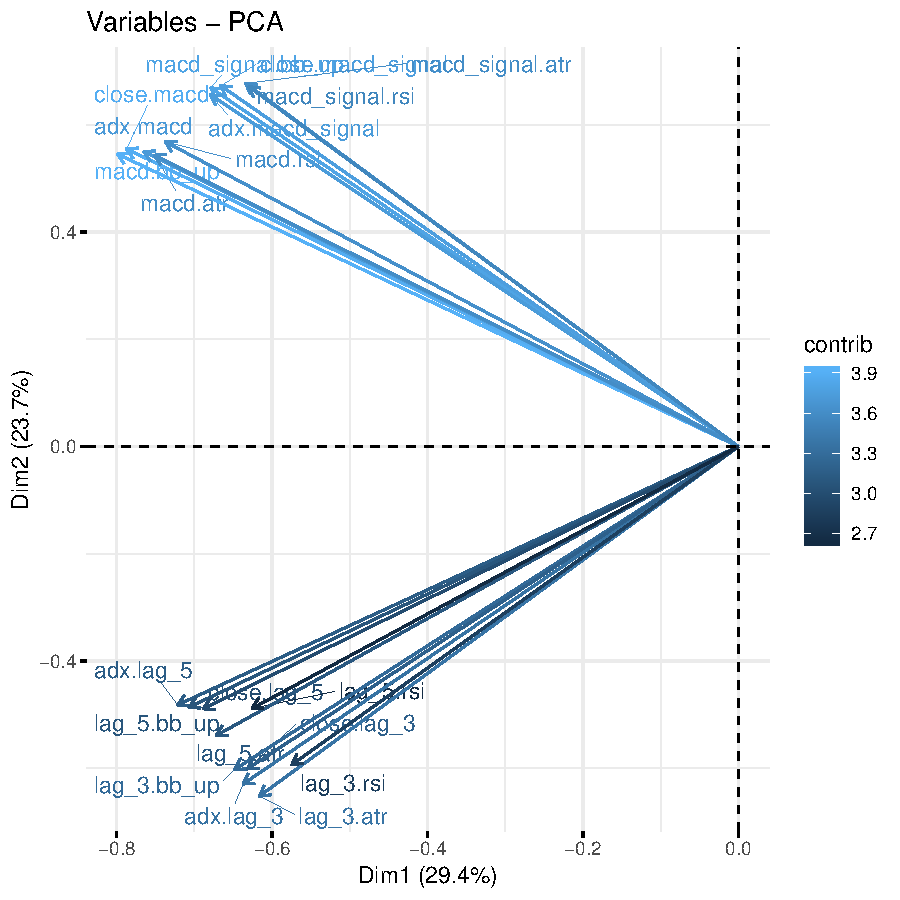
\includegraphics{main-011}
\caption{Trades según tipo de salida}
\end{figure}



\begin{figure}[H]
\setkeys{Gin}{width = 1\textwidth}
\centering
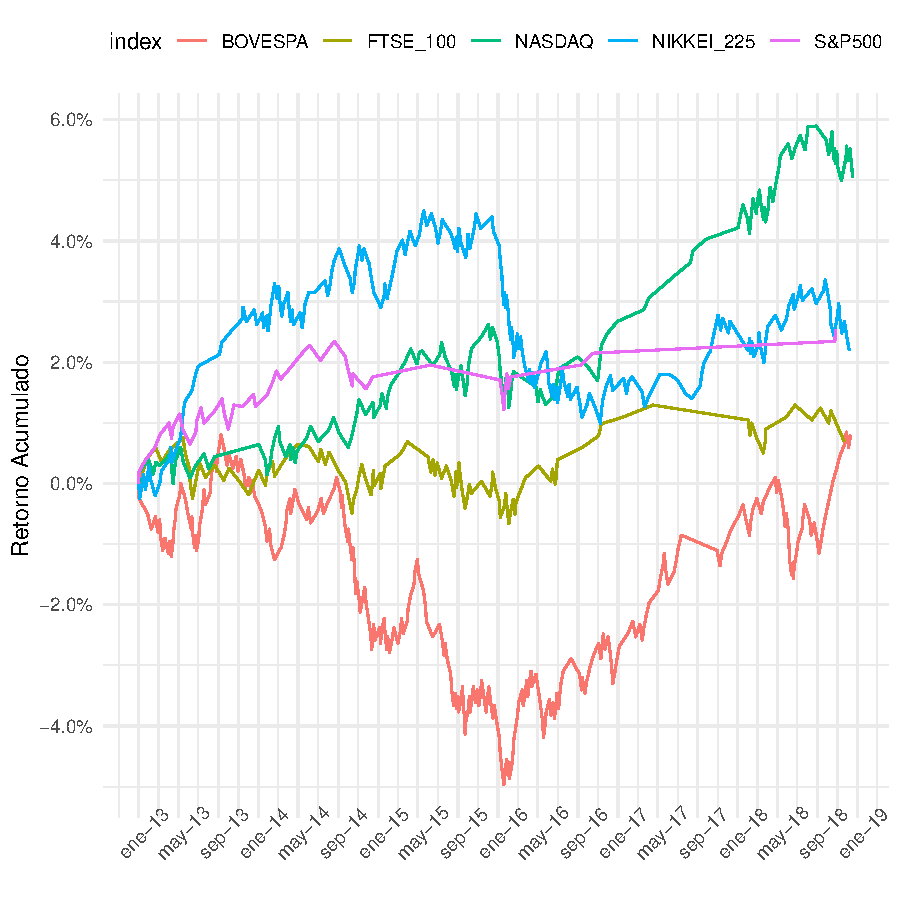
\includegraphics{main-013}
\caption{Retorno acumulado para cada índice}
\end{figure}
% !TeX root = ./main.Rnw
%\SweaveUTF8

\chapter*{Conclusiones y Recomendaciones}
\addcontentsline{toc}{chapter}{Conclusiones y Recomendaciones}



% !TeX root = ./main.Rnw
%\SweaveUTF8

\chapter*{Lista de Referencias}
\addcontentsline{toc}{chapter}{Lista de Referencias}

\begin{itemize}

\item Alexander, N. Y Zafer, D. (2016). \textit{Gestión del riesgo con el uso de commodities energéticos utilizando Valor en riesgo y Teoría del Valor Extremo}. Suecia, Universidad de Lund.

\end{itemize}

\end{document}
